\section{Use Case}
\label{sec:Use Case}
Here is a simple use case for using AstroJournal:\\
\begin{enumerate}
 \item After the first execution of AstroJournal, a default folder called AstroJournal\_files will be created in your user home folder. Inside this folder, examples of raw reports, and the default LaTeX headers / footers for each exported journals are provided. 
 \item Report your observations (with the same structure of my tsv or csv files provided in the folder raw\_reports) using a spreadsheet program, such as MS Excel, Libreoffice Spreadsheet, or Google Spreadsheet. Alternatively you can use a common text editor (e.g. Wordpad, GNU Emacs, Kate, etc.) as long as the fields are the same as in the samples provided in the raw\_report and that each field is separated using a TAB character.
 \item Export your file as tsv (if using Google Spreadsheet) or csv. In the latter case, when asked, select tab as field delimiter.
 \item Put this file in the folder raw\_reports.
 \item Start the AstroJournal application by clicking astrojournal.sh (GNU/Linux) or astrojournal.exe (Windows).
 \item Press the button ``Create Journals''.
\end{enumerate}



\subsection{Create an observation report}
\label{sec:Create an observation report}
As currently implemented, the format of the observation tables is specific. The titles (Date, Time, Location, Altitude, Temperature, Seeing, Transparency, Telescopes, Eyepieces, Filters, Target, Cons, Type, Power, and Notes) cannot be changed as these are used by AstroJournal to retrieve the data. All fields are separated by a tab character (TAB) explicitly shown in this example with a text when this must be included. Fields can have single or double quotes.\\
You can find samples of these files in the folder raw\_reports, which is 
AstroJournal input folder.\\
These files can be edited with any spreadsheet (e.g. Google SpreadSheet, MS Excel, LibreOffice SpreadSheet) or a common text editor (e.g. MS Wordpad, Emacs, Kate, or GEdit).\\
To customise the document header and footer, please look into the folder 
latex\_header\_footer to find the LaTeX files for the header and footer. Also these files can be edited with any common text editor.\\
If desired, LaTeX code can be inserted in the report. For instance, a target note could be customised as:
\begin{lstlisting}
{\color{red} Invisible} at 100x.  
\end{lstlisting}
to print the text ``{\color{red} Invisible} at 100x''. Other common customisations could be:
\begin{lstlisting}
{\bf Invisible} at 100x.  
{\it Invisible} at 100x.  
\end{lstlisting}
to print ``{\bf Invisible} at 100x'' and ``{\it Invisible} at 100x'', respectively. A combination of two could be: 
Other common customisations could be:
\begin{lstlisting}
{\color{red}\bf Invisible} at 100x.  
\end{lstlisting}
to print ``{\color{red}\bf Invisible} at 100x''.\\ 
Example of observation records contained in a file parsed by AstroJournal:\\

\begin{center}
\begin{figure}
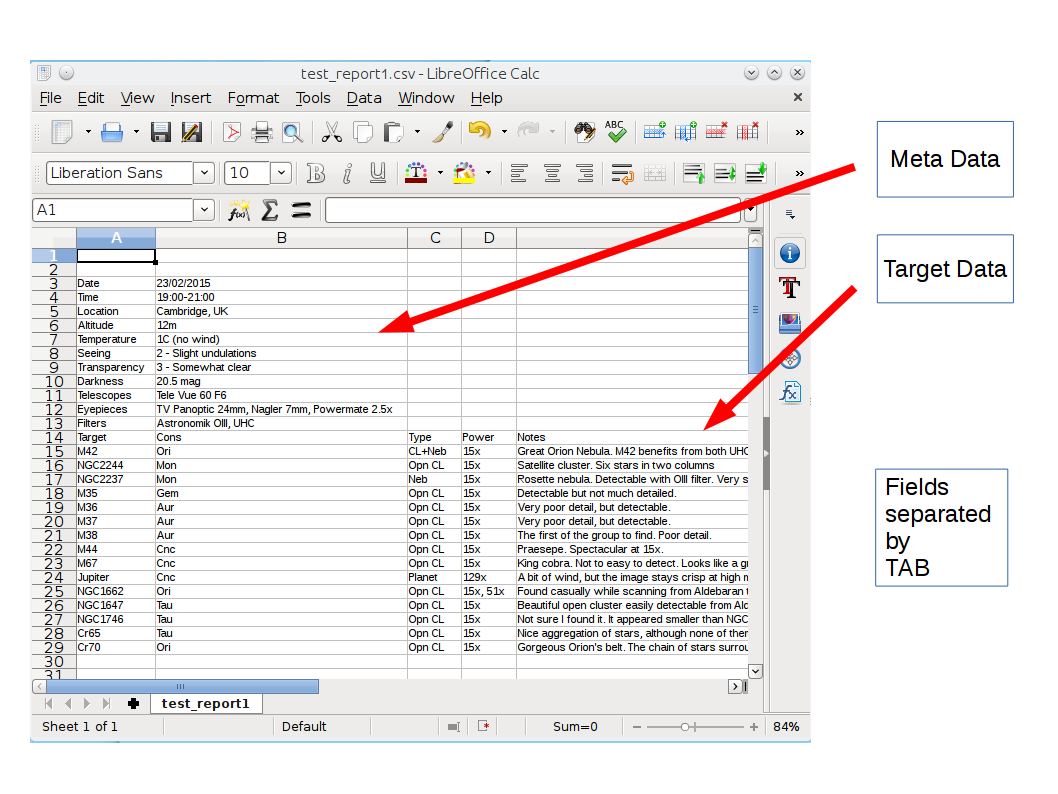
\includegraphics[width=1.2\textwidth]{images/report_sample_annot}\par\vspace{1cm}
\caption[Report example]{A report consists of two tables placed one after the other without any empty line. The first table contains the report meta data, whereas the second table lists the description for each target observed during a session. Multiple reports can be created inside the same file, but at least one empty line must be inserted between reports. When the file is exported to csv or tsv format, check that the fields are separated by a TAB delimiter.}
\end{figure}
\end{center}


